%set the master document for easy compilation
%!TEX root = ../D3_5_3.tex

\section{F2.11: manageDMI\_output}\label{s:F2.11}


\subsection{Component Requirements}

\begin{longtable}{p{.25\textwidth}p{.7\textwidth}}
\toprule
Component name			& manageDMI\_output \\
\midrule
Link to SCADE model		& {\footnotesize \url{https://github.com/openETCS/modeling/tree/master/model/Scade/System/ObuFunctions/manageData/manageDMI}} \\
\midrule
SCADE designer			& Bernd Hekele, DB Netz AG \\
\midrule
Description				& This component collects and processes outgoing messages to the Driver Machine Interface (DMI).\\
\midrule
Input documents	& 
ERA ERTMS 015560\newline
ETCS DRIVER MACHINE INTERFACE\newline
ERSA API\\
\midrule
Safety integrity level		& 4 \\
\midrule
Time constraints		& n/a \\
\midrule
API requirements 		& n/a \\
\bottomrule
\end{longtable}


\subsection{Interface}

An overview of the interface of component manageDMI\_output is shown in Figure~\ref{f:ManageDMIOutput}.  For the description of inputs and outputs we refer to the SCADE Suite model (cf. link above)  respectively the SCADE generated documentation.
%The inputs and outputs are described in detail in Section~\ref{s:ManageDMIOutput_inputs} respectively \ref{s:ManageDMIOutput_outputs}. 
Subcomponents are described in Section~\ref{s:ManageDMIOutput_subcomponents}.

\begin{figure}[H]
\center
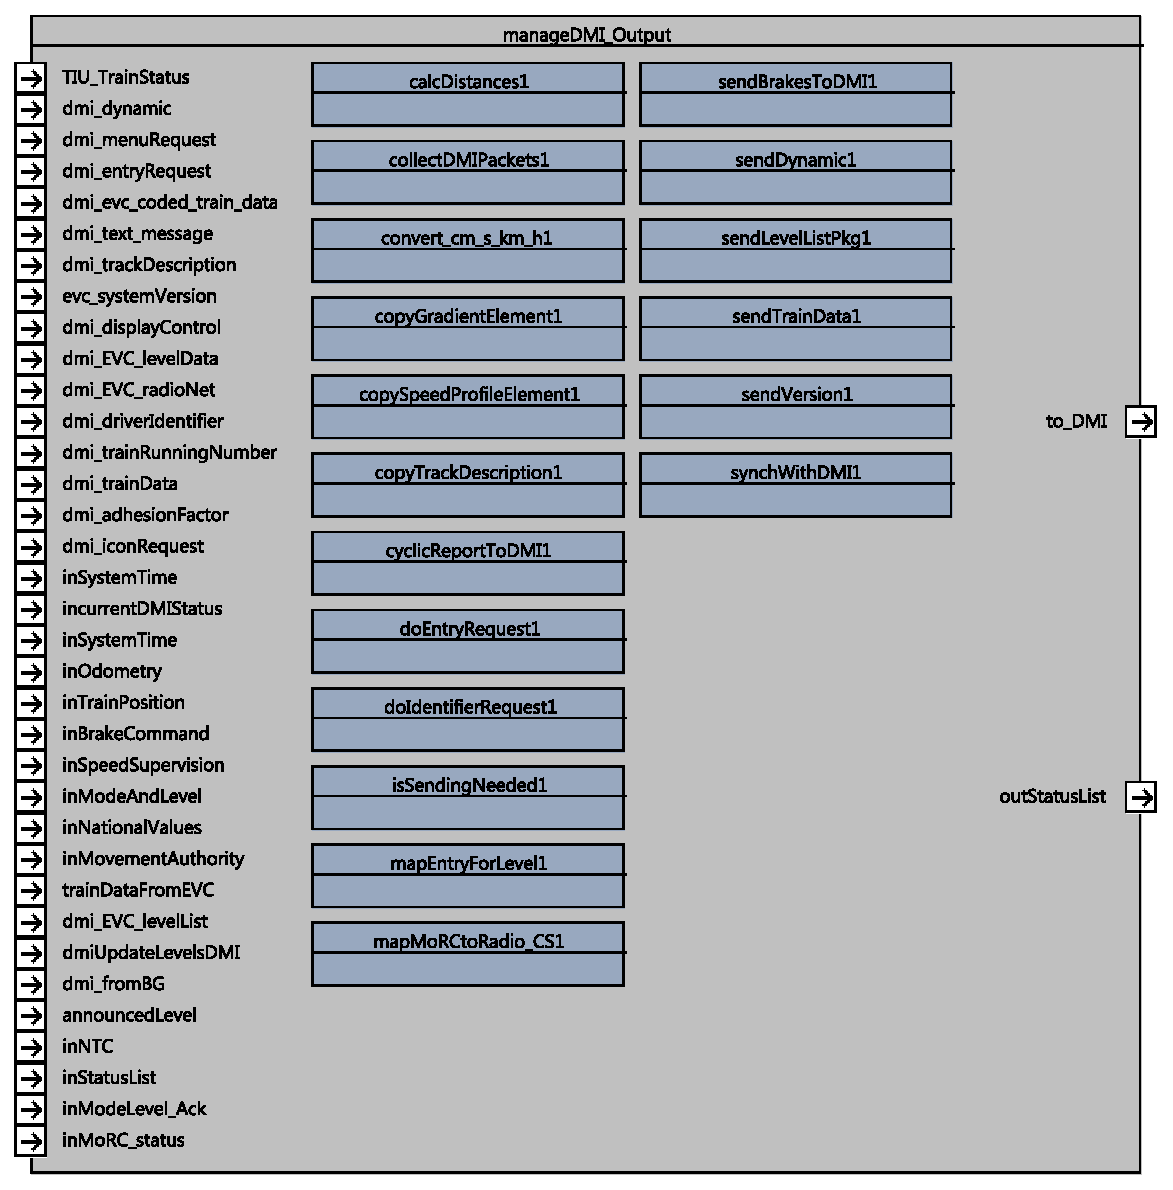
\includegraphics[width=\textwidth]{images/F2_11_manageDMI_Output.pdf}
\caption{manageDMI\_output SysML diagram.}\label{f:ManageDMIOutput}
\end{figure}

%
%\subsubsection{Inputs}\label{s:ManageDMIOutput_inputs}
%
%\paragraph{[Input 1 name]}
%
%\begin{longtable}{p{.25\textwidth}p{.7\textwidth}}
%\toprule
%Input name				& [Name of the input] \\
%\midrule
%Description				& [Brief description of the input] \\
%\midrule
%Source					& [Name of the source component] \\ 
%\midrule
%Type					& [Type of the input] \\
%\midrule
%Valid range of values	& [Complete list of valid values] \\
%\midrule
%Behaviour when value is at boundary	& [Description of components behaviour when input value is at boundary] \\
%\midrule
%Behaviour for values out of valid range	& [Description of components behaviour when input value is out of valid range] \\
%\midrule
%Behaviour when value is erroneous, absent or unwanted (i.e. spurious) & [Description of components behaviour when value is erroneous, absent or unwanted (i.e. spurious)] \\
%\bottomrule
%\end{longtable}
%
%
%\paragraph{[Input 2 name]}
%
%\begin{longtable}{p{.25\textwidth}p{.7\textwidth}}
%\toprule
%Input name				& [Name of the input] \\
%\midrule
%Description				& [Brief description of the input] \\
%\midrule
%Source					& [Name of the source component] \\ 
%\midrule
%Type					& [Type of the input] \\
%\midrule
%Valid range of values	& [Complete list of valid values] \\
%\midrule
%Behaviour when value is at boundary	& [Description of components behaviour when input value is at boundary] \\
%\midrule
%Behaviour for values out of valid range	& [Description of components behaviour when input value is out of valid range] \\
%\midrule
%Behaviour when value is erroneous, absent or unwanted (i.e. spurious) & [Description of components behaviour when value is erroneous, absent or unwanted (i.e. spurious)] \\
%\bottomrule
%\end{longtable}
%
%
%\subsubsection{Outputs}\label{s:ManageDMIOutput_outputs}
%
%\paragraph{[Output 1 name]}
%
%\begin{longtable}{p{.25\textwidth}p{.7\textwidth}}
%\toprule
%Output name				& [Name of the output] \\
%\midrule
%Description				& [Brief description of the output] \\
%\midrule
%Destination				& [Name of the destination component(s)] \\ 
%\midrule
%Type					& [Type of the output] \\
%\midrule
%Valid range of values	& [Complete list of valid values] \\
%\midrule
%Behaviour when value is at boundary	& [Description of components behaviour when output value is at boundary] \\
%\midrule
%Behaviour for values out of valid range	& [Description of components behaviour when output value is out of valid range] \\
%\midrule
%Behaviour when value is erroneous, absent or unwanted (i.e. spurious) & [Description of components behaviour when value is erroneous, absent or unwanted (i.e. spurious)] \\
%\bottomrule
%\end{longtable}
%
%
%\paragraph{[Output 2 name]}
%
%\begin{longtable}{p{.25\textwidth}p{.7\textwidth}}
%\toprule
%Output name				& [Name of the output] \\
%\midrule
%Description				& [Brief description of the output] \\
%\midrule
%Destination				& [Name of the destination component(s)] \\ 
%\midrule
%Type					& [Type of the output] \\
%\midrule
%Valid range of values	& [Complete list of valid values] \\
%\midrule
%Behaviour when value is at boundary	& [Description of components behaviour when output value is at boundary] \\
%\midrule
%Behaviour for values out of valid range	& [Description of components behaviour when output value is out of valid range] \\
%\midrule
%Behaviour when value is erroneous, absent or unwanted (i.e. spurious) & [Description of components behaviour when value is erroneous, absent or unwanted (i.e. spurious)] \\
%\bottomrule
%\end{longtable}

\subsection{Subcomponents}\label{s:ManageDMIOutput_subcomponents}


\subsubsection{cyclicReportToDMI}
%set the master document for easy compilation
%!TEX root = ../D3_5_3.tex

\paragraph{Component Requirements}

\begin{longtable}{p{.25\textwidth}p{.7\textwidth}}
\toprule
Component name			& cyclicReportToDMI \\
\midrule
Link to SCADE model		& {\footnotesize \url{https://github.com/openETCS/modeling/tree/master/model/Scade/System/ObuFunctions/manageData/manageDMI}} \\
\midrule
SCADE designer			& Bernd Hekele, DB Netz AG \\
\midrule
Description				& This subcomponent is responsible for writing and sending Dynamic Packets to the DMI. \\
\midrule
Input documents	& 
ERA ERTMS 015560\newline
ETCS DRIVER MACHINE INTERFACE\newline
ERSA API\\
\midrule
Safety integrity level	& 4 \\
\midrule
Time constraints		& periodically \\
\midrule
API requirements 		& n/a\\
\bottomrule
\end{longtable}


\paragraph{Interface}

For an overview of the interface of this internal component we refer to the SCADE model (cf.~link above) respectively the SCADE generated documentation.

\subsubsection{ManageTextMessages}
%set the master document for easy compilation
%!TEX root = ../D3_5_3.tex

\paragraph{Component Requirements}

\begin{longtable}{p{.25\textwidth}p{.7\textwidth}}
\toprule
Component name			& ManageTextMessages \\
\midrule
Link to SCADE model		& {\footnotesize \url{https://github.com/openETCS/modeling/tree/master/model/Scade/System/ObuFunctions/manageData/manageDMI}} \\
\midrule
SCADE designer			& Bernd Hekele, DB Netz AG \\
\midrule
Description				& This subcomponent receives available text messages from within the EVC sources, handles messages according to the priority, and provides an output stack for messages. \\
\midrule
Input documents			& 
ERA ERTMS 015560\newline
ETCS DRIVER MACHINE INTERFACE\newline
ERSA API\\
\midrule
Safety integrity level	& 4 \\
\midrule
Time constraints		&  n/a \\
\midrule
API requirements 		&  n/a \\
\bottomrule
\end{longtable}


\paragraph{Interface}

For an overview of the interface of this internal component we refer to the SCADE model (cf.~link above) respectively the SCADE generated documentation.

\subsubsection{copyTrackDescription}
%set the master document for easy compilation
%!TEX root = ../D3_5_3.tex

\paragraph{Component Requirements}

\begin{longtable}{p{.25\textwidth}p{.7\textwidth}}
\toprule
Component name			& copyTrackDescription \\
\midrule
Link to SCADE model		& {\footnotesize \url{http://???}} \\
\midrule
SCADE designer			& [Name, affiliation] \\
\midrule
Description				& [Brief description of functionality] \\
\midrule
Input documents	& 
Subset-026, Chapter ?.?\newline
Subset-026, Chapter ?.?\newline
Subset-026, Chapter ?.?.?\\
\midrule
Safety integrity level	& 4 \\
\midrule
Time constraints		& [If applicable description of time constraints, otherwise n/a] \\
\midrule
API requirements 		& [If applicable description of API requirements, otherwise n/a] \\
\bottomrule
\end{longtable}


\paragraph{Interface}

For an overview of the interface of this internal component we refer to the SCADE model (cf.~link above) respectively the SCADE generated documentation.

%\subsubsection{toEntryRequest}
%%set the master document for easy compilation
%!TEX root = ../D3_5_3.tex

\paragraph{Component Requirements}

\begin{longtable}{p{.25\textwidth}p{.7\textwidth}}
\toprule
Component name			& toEntryRequest \\
\midrule
Link to SCADE model		& {\footnotesize \url{http://???}} \\
\midrule
SCADE designer			& Bernd Hekele, DB Netz AG \\
\midrule
Description				& [Brief description of functionality] \\
\midrule
Input documents	& 
Subset-026, Chapter ?.?\newline
Subset-026, Chapter ?.?\newline
Subset-026, Chapter ?.?.?\\
\midrule
Safety integrity level	& 4 \\
\midrule
Time constraints		& [If applicable description of time constraints, otherwise n/a] \\
\midrule
API requirements 		& [If applicable description of API requirements, otherwise n/a] \\
\bottomrule
\end{longtable}


\paragraph{Interface}

For an overview of the interface of this internal component we refer to the SCADE model (cf.~link above) respectively the SCADE generated documentation.
%
%\subsubsection{sendBrakesToDMI}
%%set the master document for easy compilation
%!TEX root = ../D3_5_3.tex

\paragraph{Component Requirements}

\begin{longtable}{p{.25\textwidth}p{.7\textwidth}}
\toprule
Component name			& sendBrakesToDMI \\
\midrule
Link to SCADE model		& {\footnotesize \url{http://???}} \\
\midrule
SCADE designer			& [Name, affiliation] \\
\midrule
Description				& [Brief description of functionality] \\
\midrule
Input documents	& 
Subset-026, Chapter ?.?\newline
Subset-026, Chapter ?.?\newline
Subset-026, Chapter ?.?.?\\
\midrule
Safety integrity level	& 4 \\
\midrule
Time constraints		& [If applicable description of time constraints, otherwise n/a] \\
\midrule
API requirements 		& [If applicable description of API requirements, otherwise n/a] \\
\bottomrule
\end{longtable}


\paragraph{Interface}

For an overview of the interface of this internal component we refer to the SCADE model (cf.~link above) respectively the SCADE generated documentation.

%\subsubsection{manageDMI\_Output}
%%set the master document for easy compilation
%!TEX root = ../D3_5_3.tex

\paragraph{Component Requirements}

\begin{longtable}{p{.25\textwidth}p{.7\textwidth}}
\toprule
Component name			& manageDMI\_Output \\
\midrule
Link to SCADE model		& {\footnotesize \url{http://???}} \\
\midrule
SCADE designer			& [Name, affiliation] \\
\midrule
Description				& [Brief description of functionality] \\
\midrule
Input documents	& 
Subset-026, Chapter ?.?\newline
Subset-026, Chapter ?.?\newline
Subset-026, Chapter ?.?.?\\
\midrule
Safety integrity level	& 4 \\
\midrule
Time constraints		& [If applicable description of time constraints, otherwise n/a] \\
\midrule
API requirements 		& [If applicable description of API requirements, otherwise n/a] \\
\bottomrule
\end{longtable}


\paragraph{Interface}

For an overview of the interface of this internal component we refer to the SCADE model (cf.~link above) respectively the SCADE generated documentation.

%\subsubsection{sendTrainData}
%%set the master document for easy compilation
%!TEX root = ../D3_5_3.tex

\paragraph{Component Requirements}

\begin{longtable}{p{.25\textwidth}p{.7\textwidth}}
\toprule
Component name			& sendTrainData \\
\midrule
Link to SCADE model		& {\footnotesize \url{http://???}} \\
\midrule
SCADE designer			& Bernd Hekele, DB Netz AG \\
\midrule
Description				& [Brief description of functionality] \\
\midrule
Input documents	& 
Subset-026, Chapter ?.?\newline
Subset-026, Chapter ?.?\newline
Subset-026, Chapter ?.?.?\\
\midrule
Safety integrity level	& 4 \\
\midrule
Time constraints		& [If applicable description of time constraints, otherwise n/a] \\
\midrule
API requirements 		& [If applicable description of API requirements, otherwise n/a] \\
\bottomrule
\end{longtable}


\paragraph{Interface}

For an overview of the interface of this internal component we refer to the SCADE model (cf.~link above) respectively the SCADE generated documentation.

%\subsubsection{sendVersion}
%%set the master document for easy compilation
%!TEX root = ../D3_5_3.tex

\paragraph{Component Requirements}

\begin{longtable}{p{.25\textwidth}p{.7\textwidth}}
\toprule
Component name			& sendVersion \\
\midrule
Link to SCADE model		& {\footnotesize \url{http://???}} \\
\midrule
SCADE designer			& Bernd Hekele, DB Netz AG \\
\midrule
Description				& [Brief description of functionality] \\
\midrule
Input documents	& 
Subset-026, Chapter ?.?\newline
Subset-026, Chapter ?.?\newline
Subset-026, Chapter ?.?.?\\
\midrule
Safety integrity level	& 4 \\
\midrule
Time constraints		& [If applicable description of time constraints, otherwise n/a] \\
\midrule
API requirements 		& [If applicable description of API requirements, otherwise n/a] \\
\bottomrule
\end{longtable}


\paragraph{Interface}

For an overview of the interface of this internal component we refer to the SCADE model (cf.~link above) respectively the SCADE generated documentation.
%
%\subsubsection{sendLevelListPkg}
%%set the master document for easy compilation
%!TEX root = ../D3_5_3.tex

\paragraph{Component Requirements}

\begin{longtable}{p{.25\textwidth}p{.7\textwidth}}
\toprule
Component name			& sendLevelListPkg \\
\midrule
Link to SCADE model		& {\footnotesize \url{http://???}} \\
\midrule
SCADE designer			& [Name, affiliation] \\
\midrule
Description				& [Brief description of functionality] \\
\midrule
Input documents	& 
Subset-026, Chapter ?.?\newline
Subset-026, Chapter ?.?\newline
Subset-026, Chapter ?.?.?\\
\midrule
Safety integrity level	& 4 \\
\midrule
Time constraints		& [If applicable description of time constraints, otherwise n/a] \\
\midrule
API requirements 		& [If applicable description of API requirements, otherwise n/a] \\
\bottomrule
\end{longtable}


\paragraph{Interface}

For an overview of the interface of this internal component we refer to the SCADE model (cf.~link above) respectively the SCADE generated documentation.







